\chapter{Modelling, Data, and Simulation}
\label{cha:model}

\minitoc

After describing the state-of-the-art, this Section presents the models, data, and simulation tools used in this thesis. First, we focus on the model describing the offline and online modules. We explain what kind of information is exchanged between offline and online. Also, we detail the power, scheduling, and server decisions. After the model, we introduce the traces used in the experiments. These traces emulates a real environment regarding workload, weather, and platform. Finally, we demonstrate the simulation tools.

\section{Model}

As presented in Chapter \ref{cha:related_work}, a gap in the state-of-the-art is the mix of offline and online. Figure \ref{fig:model} illustrates the architecture proposed by the Datazero2 project, mixing both decision levels \cite{Datazero}. Since this work is part of the Datazero2 project, we use the same architecture. There are four main modules: IT Decision Module (ITDM), Power Decision Module (PDM), Negotiation Module (NM), and Online Decision Module (ODM). ITDM, PDM, and NM are responsible for the offline decisions, and ODM manages the online actions. This thesis focuses on the Online Decision Module, but we present in the following sections the optimizations made in offline modules to provide the data needed by ODM. 

\begin{figure}[!htb]
    \centering
    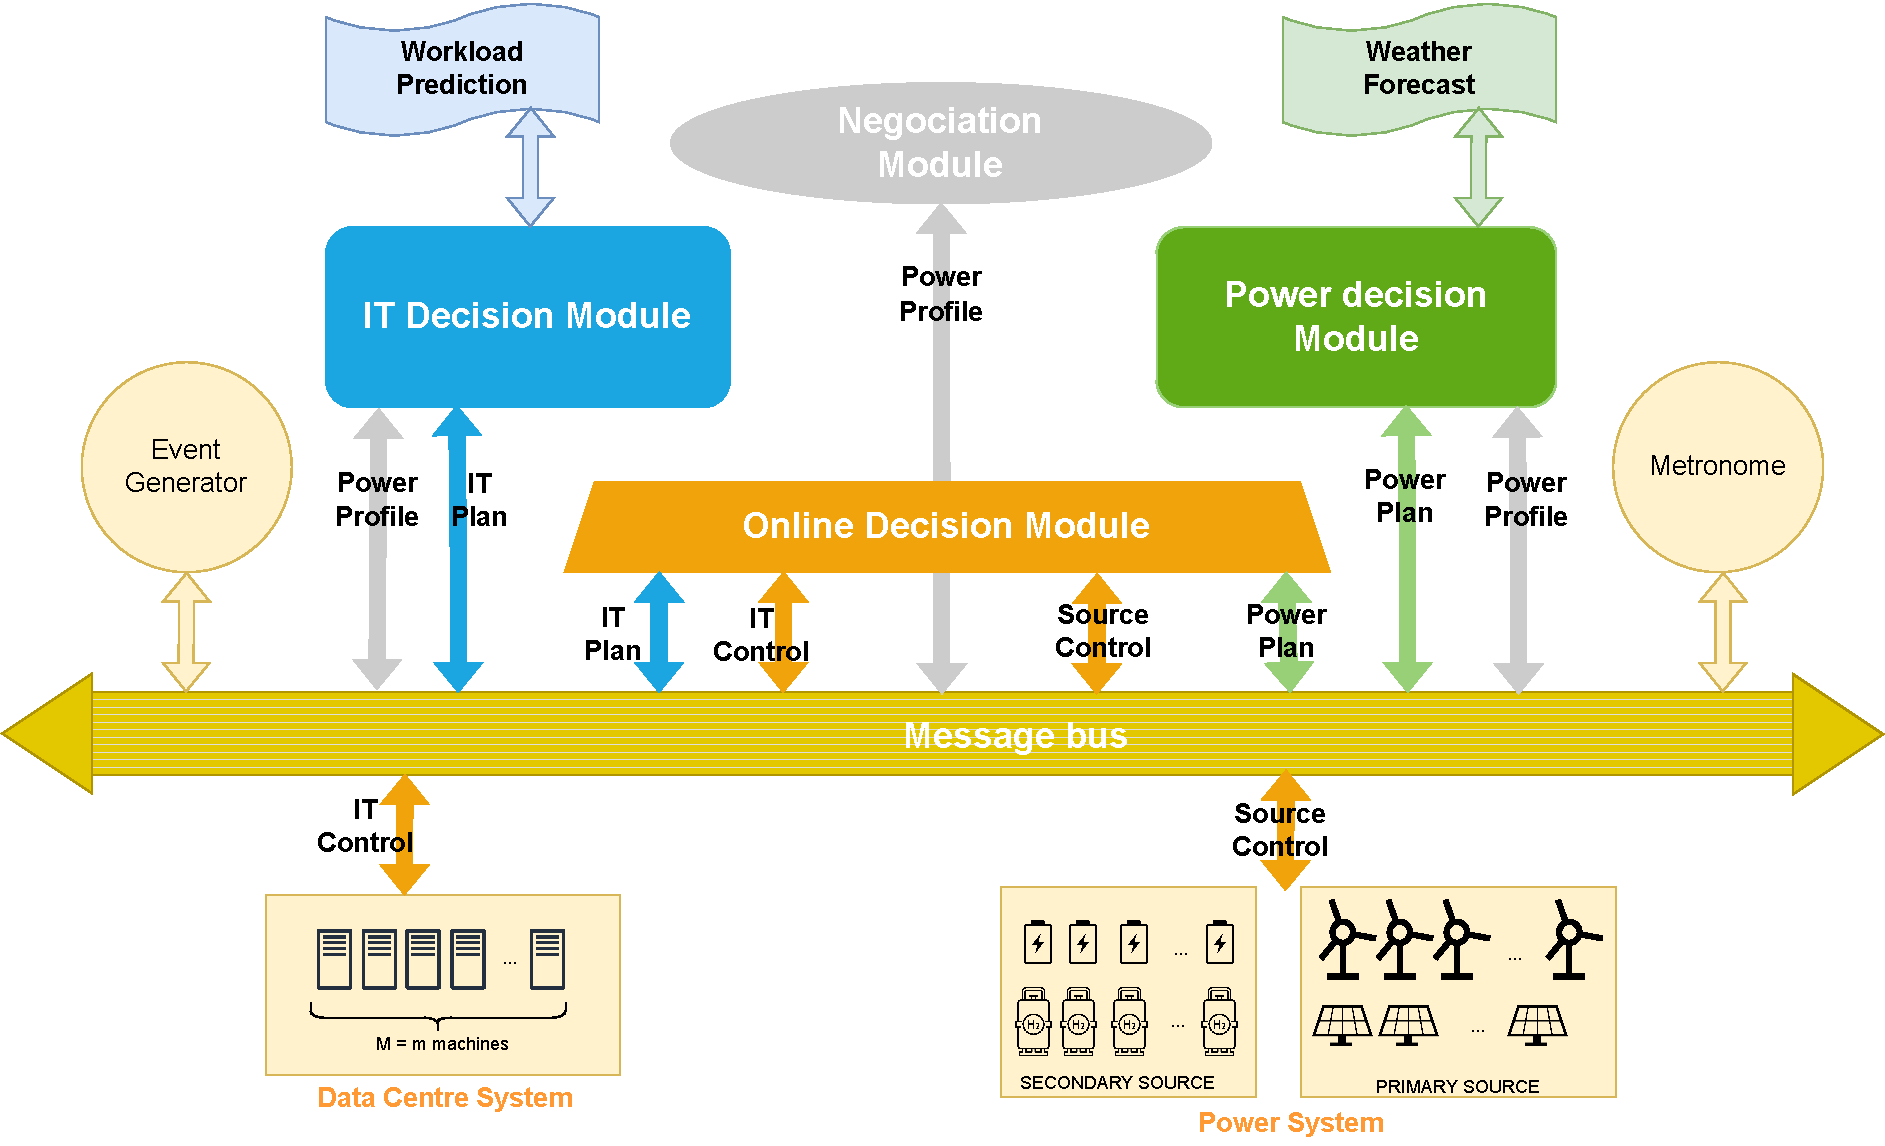
\includegraphics[scale=0.45]{Images/Model/model.pdf}
    \caption{Datazero2 architecture \cite{Datazero}.}
    \label{fig:model}
\end{figure}

Besides these four modules, Datazero2 also includes an event generator and metronome. Both components are essential for the simulations. Event generator simulates the real events of a data center, such as job submission, weather conditions, etc. It simply reads a file and sends the data to the bus. The metronome synchronizes the simulation, managing the clock. So, every component waits for the time evolution from the metronome. This thesis does not detail these components, concentrating on the decision modules and their interactions.

Table \ref{tab:notation_system} presents the general notations and each following section introduces its own notations. Both offline and online use the time division from Figure \ref{fig:time_window}. The time window is the horizon of the offline plan. Offline considers the time window to define how far to predict weather and workload. Also, it uses the time window to determine the power and server configuration plan duration. Our model divides the time window into several time steps, as represented in Figure \ref{fig:time_window} by the different $t$. The actions for power and server are constant inside the time step. For example, if a server is at some state in step $t=0$, it will remain at this state during the step duration.

\begin{table*}[!htb]
\centering
% \scriptsize
\caption{General notations.}
\label{tab:notation_system}
\begin{tabular}{l|l}
    \hline
    Notation & Description \\\hline\hline
    % System
    $t$ & Time step (int)\\
    $T$ & Last time step (int)\\
    $\Delta t$ & Time step length (s)\\
    $T_{w}$ & Time window length (s)\\
    $P_{load}$ & Estimated power demand (kW)\\
    $u_{load}$ & Uncertainty of $P_{load}$\\
    $P_{prod}$ & Power production by all sources (kW)\\
    $P_{renew}$ & Power delivered by renewable sources (kW)\\
    $u_{renew}$ & Uncertainty of $P_{renew}$\\
    \hline
\end{tabular}
\end{table*}

\begin{figure}[!htb]
    \centering
    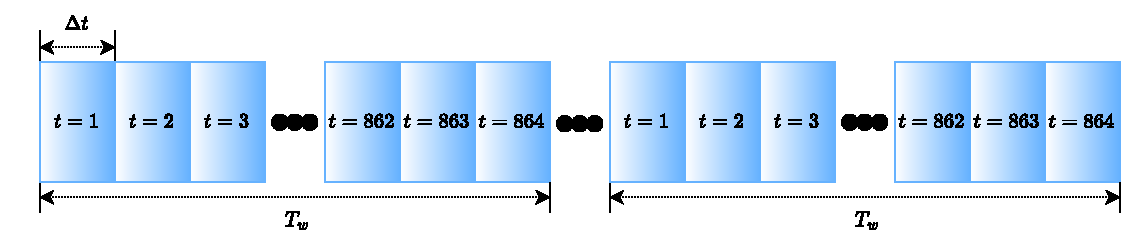
\includegraphics[scale=0.75]{Images/Model/Time window.pdf}
    \caption{Time window definition.}
    \label{fig:time_window}
\end{figure}

\subsection{Offline Decision Modules}
This section starts presenting the offline decision module. First, we demonstrate how PDM and ITDM agree on a power envelope (through NM). Then, we explain the power decisions from PDM, resulting in a power plan. Finally, we detail the ITDM, which defines the IT plan.

\subsubsection{Negotiation (NM)}
Negotiation is a crucial step in Datazero2 architecture. A renewable-only data center introduces several constraints and decision variables. On the PDM side, it must approximate demand and production while considering long-term storage elements. For example, PDM can provide more power from hydrogen in a case with low renewable generation. However, PDM must evaluate the impact of its actions since the energy of the storage is finite. On the other hand, ITDM maximizes the Quality of Service. Thus, it demands more energy to run more servers at faster speeds. NM is between PDM and ITDM, trying to find an agreement. NM works iteratively. On each iteration, both PDM and ITDM propose a power envelope to NM, considering the objective of each module. A power envelope is a time series of the power production from the sources in a time window. While PDM tries to reduce the power envelope to control the storage, ITDM increases it to run more jobs faster. NM compares both envelope propositions and returns a new one. Then, each module verifies if they can use the proposed power envelope. They run several iterations until both agree or reach a timeout.

Since this thesis focus on the online part, we simplify this process. We implemented the negotiation in three steps. First, ITDM proposes a power envelope $P_{load}$ based on the energy demanded to run a predicted workload. Then, PDM takes this envelope and runs its optimization. It can degrade the power envelope to meet its objectives, resulting in a new power envelope $P_{prod}$. Finally, ITDM takes the PDM power production and finds the best server configuration that meets it. The following sections present the PDM and ITDM optimizations.

\subsubsection{Power Decision Module (PDM)}
Table \ref{tab:notation_power} gives the notations for PDM. PDM plans the renewable source engagement to provide the energy needed to maintain the IT elements. A renewable-only data center introduces several constraints in power generation. Therefore, PDM must approximate the demanded power while considering long-term storage elements. For example, it can use more energy coming from hydrogen during the winter, which has lower power production, compensating for this usage in the summer, which has higher power generation. On the other hand, PDM can degrade the provided energy due to a lack of energy from storage and estimated renewable. In the context of Datazero, \citeauthor{haddad2019mixed} created the first model to solve this problem \cite{haddad2019mixed}. This thesis uses a similar model to PDM. Equation \ref{equ:model_energy} gives the power production from all renewable sources. Equation \ref{equ:renewable_power} indicates that $P_{renew}$ comes from wind and solar production. $P_{wt}(t)$, $P_{pv}(t)$, $P_{fc}(t)$, $P_{ez}(t)$, $P_{dch}(t)$, and $P_{ch}(t)$ are calculated using Equations \ref{equ:wind_turbines}, \ref{equ:panel_solar_with_temperature}, \ref{equ:hydrogen_full_cell}, \ref{equ:hydrogen_electrolyzer} and \ref{equ:battery_energy} from Section \ref{sec:related_work_electrical_elements}.

\begin{table*}[!htb]
\centering
% \scriptsize
\caption{Notations for PDM.}
\label{tab:notation_power}
\begin{tabular}{l|l}
    \hline
    Notation & Description \\\hline\hline
    % Power
    $P_{wt}$ & Power delivered by wind turbines (kW)\\
    $P_{pv}$ & Power delivered by solar panels (kW)\\
    $P_{fc}$ & Power delivered by fuel cell (kW)\\
    $P_{ez}$ & Power put into electrolyzer to generate hydrogen (kW)\\
    $P_{dch}$ & Battery discharging power (kW)\\
    $P_{ch}$ & Battery charging power (kW)\\
    $\eta_{ch}$ & Battery charge efficiency (\%)\\
    $\eta_{dch}$ & Battery discharge efficiency (\%)\\
    $SoC$ & State of Charge (\%)\\
    $LoH$ & Level of Hydrogen (kg)\\
    $SoC_{max}$ & Maximal battery State of Charge (\%)\\
    $SoC_{min}$ & Minimal battery State of Charge (\%)\\
    $B_{size}$ & Size of the battery (kWh)\\
    $LoH_{max}$ & H2 tank limit (kg)\\
    $P_{dch_{max}}$ & Battery maximum discharging power (kW)\\
    $P_{ch_{max}}$ & Battery maximum charging power (kW)\\
    $P_{fc_{max}}$ & Fuel cell maximum charging power (kW)\\
    $P_{ez_{min}}$ & Electrolyzer minimum charging power (kW)\\
    $P_{ez_{max}}$ & Electrolyzer maximum charging power (kW)\\
    $SoC_{target}$ & Target State of Charge at the end of the time window (\%)\\
    $LoH_{target}$ & Target Level of Hydrogen at the end of the time window (kg)\\
    $rf$ & Relax factor (float) \\
    $P^{real}_{load}$ & Real power demand (kW)\\
    $P^{real}_{renew}$ & Estimated power demand (kW)\\
    \hline
\end{tabular}
\end{table*}

\begin{equation}
    \label{equ:model_energy}
    P_{prod}(t) = P_{renew}(t) + (P_{fc}(t) + P_{dch}(t) - P_{ez}(t) - P_{ch}(t)), \quad \forall 0 \le t \le T
\end{equation}

\begin{equation}
    \label{equ:renewable_power}
    P_{renew}(t) = P_{wt}(t) + P_{pv}(t), \quad \forall 0 \le t \le T
\end{equation}

$P_{ch}(t)$, $P_{dch}(t)$, $P_{ez}(t)$, and $P_{fc}(t)$ are the decision variables in Equation \ref{equ:model_energy}, since $P_{wt}(t)$ and $P_{pv}(t)$ come from wind speed and solar irradiation. As presented in Section \ref{sec:related_work_electrical_elements}, $SoC(t)$ depends on the charge $P_{ch}(t)$ and discharge $P_{dch}(t)$ (see Equation \ref{equ:battery_energy}), and $LoH(t)$ depends on the power of the electrolyzer $P_{ez}(t)$ and fuel cells $P_{fc}(t)$ (see Equation \ref{equ:hydrogen_level}). Regarding $SoC(t)$, the state of charge must be between the boundaries $SoC_{min}$ and $SoC_{max}$, as demonstrated in Equation \ref{equ:battery_boundaries}. These boundaries help to extend the battery life \cite{xu2016modeling}.

\begin{equation}
    \label{equ:battery_boundaries}
    SoC_{min} \leq SoC(t) \leq SoC_{max}, \quad \forall 0 \le t \le T
\end{equation}

On the other hand, hydrogen only has the tank size as a boundary. So, Equation \ref{equ:hydrogen_boundaries} presents the level of hydrogen constraint.

\begin{equation}
    \label{equ:hydrogen_boundaries}
    0 \leq LoH(t) \leq LoH_{max}, \quad \forall 0 \le t \le T
\end{equation}

Considering the power to charge/discharge, both have upper limits. These boundaries avoid destroying the battery. So, we introduce constraints \ref{equ:discharge_boundary} and \ref{equ:charge_boundary}.

\begin{equation}
    \label{equ:discharge_boundary}
    0 \leq P_{dch}(t) \leq P_{dch_{max}}, \quad \forall 0 \le t \le T
\end{equation}

\begin{equation}
    \label{equ:charge_boundary}
    0 \leq P_{ch}(t) \leq P_{ch_{max}}, \quad \forall 0 \le t \le T
\end{equation}

Fuel cells and electrolyzers also have boundaries. While fuel cells have only a maximum limit, electrolyzers have an operating range. So, Equations \ref{equ:fuelcells_boundary} and \ref{equ:electrolyzer_boundary} present them.

\begin{equation}
    \label{equ:fuelcells_boundary}
    0 \leq P_{fc}(t) \leq P_{fc_{max}}, \quad \forall 0 \le t \le T
\end{equation}

\begin{equation}
    \label{equ:electrolyzer_boundary}
    P_{ez_{min}} \leq P_{ez}(t) \leq P_{ez_{max}}, \quad \forall 0 \le t \le T
\end{equation}

Another important constraint is the target hydrogen and battery level at the end of the time window. Using only the previous constraints, the model can use all the power available in the energy storages, drying them but providing a high quality of service. However, Figure \ref{fig:time_window} shows that the time windows are chained. So, the next time window will not have energy in the storage. Therefore, we introduce these targets. So, the state of charge and level of hydrogen in the last step of the time window must respect Equations \ref{equ:soc_target} and \ref{equ:loh_target}. These targets can be the subject of another optimization or indicated by hand by the data center manager. Also, the targets must consider the long-term perspective, such as seasons with lower/higher production, the peak of demand over an external event, etc. 

\begin{equation}
    \label{equ:soc_target}
    SoC(T) \ge SoC_{target}
\end{equation}

\begin{equation}
    \label{equ:loh_target}
    LoH(T) \ge LoH_{target}
\end{equation}

Finally, the objective is to approximate the power production to the power demand. So, Equation \ref{equ:load_production} shows the relation between demand ($P_{load}$) and generation ($P_{prod}$). The optimization finds a solution where the production is higher or equal to the demand. However, it can not match both in every case. Therefore, the model introduces a demand degradation using a relax factor ($rf$). With the relax factor equal to 0, it matches demand and production. Increasing the relax factor would reduce the power given to IT, impacting the QoS. Thus, the objective is reducing the relax factor, as presented in Equation \ref{equ:objective_function}.

\begin{equation}
    \label{equ:load_production}
    P_{prod}(t) \ge (1 - rf) \times P_{load}, \quad \forall 0 \le t \le T
\end{equation}

\begin{equation}
    \label{equ:objective_function}
    \mathbf{minimize}\ rf
\end{equation}

% \citeauthor{haddad2019mixed} presented a way to linearize this model, allowing it to be solved using MILP. This thesis used the \citeauthor{haddad2019mixed} proposition to solve it using MILP. 

% \begin{equation}
%     \label{equ:model_wind_turbines}
%     P_{WT}(t) = \begin{cases}
%         0 & v \leq v_{in} \text{ or } v(t) > v_{out} \\
%         P_{WT,rated} \times \frac{v^{3}(t) - v^{3}_{in}}{v^{3}_{rated} - v^{3}_{in}} & v_{in} < v(t) \leq v_{rated} \\
%         P_{WT,rated} & v_{rated} < v(t) \leq v_{out}
%     \end{cases}
% \end{equation}

% \begin{equation}
%     \label{equ:model_panel_solar_with_temperature}
%     P_{pv}(t) = P_{R,PV} \times (R / R_{ref}) \times \eta_{PV}
% \end{equation}

% \begin{equation}
%     \label{equ:model_battery_energy}
%     E_{bat}(t) = (E_{bat}(t-1) \times (1 - \sigma)) + (P_{ch}(t-1) \times \eta_{ch} \times \Delta t) - (P_{dch}(t-1) \times \eta_{dch} \times \Delta t)
% \end{equation}
% \begin{equation}
%     \label{equ:model_battery_state_of_charge}
%     SoC(t) = \frac{E_{bat}(t)}{B_{size}} \times 100
% \end{equation}

% \begin{equation}
%     \label{equ:model_hydrogen_electrolyzer}
%     P_{ez}(t) \times \Delta t = \frac{HH_{h_{2}} \times Q_{ez}(t)}{\eta_{ez}}
% \end{equation}

% \begin{equation}
%     \label{equ:model_hydrogen_full_cell}
%     P_{fc}(t) \times \Delta t = LH_{h_{2}} \times Q_{fc}(t) \times \eta_{fc}
% \end{equation}

% \begin{equation}
%     \label{equ:model_hydrogen_level}
%     LoH(t) = LoH(t-1) + Q_{ez}(t-1) - Q_{fc}(t-1)
% \end{equation}

\subsubsection{IT Decision Module (ITDM)}

Table \ref{tab:notation_it} introduces the notations for ITDM. Following PDM optimization, ITDM aims to maximize QoS, translating $P_{prod}(t)$ into server configuration. Server configuration means the CPU P-state of the servers. For each P-state, the server has a speed (in flops \cite{hunger2005floating}) and power consumption (in W). Table \ref{tab:servers} exemplifies this relation. The CPU frequency range is discrete, although some works define it to be continuous \cite{saha2012experimental}. ITDM must find the best combination of servers off and on at some speed that uses equal or less energy than the power envelope $P_{prod}(t)$. Thus, given a data center with $S$ servers, each server $s$ has a list of states $D_s$. Each state $d$ in $D_s$ has a speed $F_{s,d}$ and a power $P_{s,d}$. $D_{s,d}(t)$ is the boolean decision variable that indicates that the server $s$ is at state $d$ at step $t$. The sleep state has a different state $Dsl_{s}(t)$ which helps to identify the transition between sleeping and running. The transition between on$\rightarrow$off is called sedating and off$\rightarrow$on is waking.

\begin{table*}[!htb]
\centering
% \scriptsize
\caption{Notations for ITDM.}
\label{tab:notation_it}
\begin{tabular}{l|l}
    \hline
    Notation & Description \\\hline\hline
    $S$ & Servers (list) \\
    $N_{S}$ & Number of servers (int) \\
    $s$ & Server index (int) \\
    $D_s$ & States of server s (list) \\
    $N_{D_{s}}$ & Number of states of server s (int) \\
    $d$ & State index (int) \\
    $F_{s,d}$ & Speed of server $s$ at state $d$ (Flops)\\
    $P_{s,d}$ & Power of server $s$ at state $d$ (W)\\
    $D_{s,d}$ & Indicates that the server $s$ is at state $d$ (boolean)\\
    $Dsl_{s}$ & Indicates that the server $s$ is sleeping (boolean)\\
    $wa_s$ & Indicates if the server is waking, transiting from off$\rightarrow$on (boolean) \\
    $T_{wa_s}$ & Transition time from off$\rightarrow$on (s) \\
    $se_s$ & Indicates if the server is being sedate, transiting from on$\rightarrow$off (boolean) \\
    $T_{se_s}$ & Transition time from on$\rightarrow$off (s) \\    
    $E_{tot}$ & Energy total spent by the servers (J) \\
    $E_{run}$ & Energy spent by the running servers (J) \\
    $E_{wak}$ & Energy spent by waking the servers (J) \\
    $E_{sed}$ & Energy spent by sedating the servers (J) \\
    $E_{sle}$ & Energy spent by the sleeping servers (J) \\
    \hline
\end{tabular}
\end{table*}

\begin{table}[!htb]
\centering
\caption[Server definition example]{Server definition example. The power is for all server's processors busy. The values are from Grid5000's Parasilo server~\cite{dacosta:hal-03453537v1, dacostakeynote}.}
\label{tab:servers}
\begin{tabular}{c|c|c}
    \hline
    State        & Power (W) & Speed (Gflops) \\ \hline\hline
    0                       & 221.77                   & 38.4                          \\
    1                       & 216.77                   & 37.78                         \\
    2                       & 213.58                   & 36.93                         \\
    3                       & 208.90                   & 36.01                         \\
    4                       & 204.45                   & 34.72                         \\
    5                       & 200.62                   & 33.90                         \\
    6                       & 197.28                   & 32.84                         \\
    7                       & 192.49                   & 31.72                         \\
    8                       & 184.26                   & 30.63                         \\
    9                       & 182.04                   & 29.25                         \\
    10                      & 179.75                   & 27.93                         \\
    11                      & 176.70                   & 26.37                         \\
    12                      & 175.53                   & 25.01                         \\
    13 (sleep)              & 4.5                      & 0                             \\ \hline
\end{tabular}
\end{table}

First, Equation \ref{equ:one_state_only} ensures only one state per time $t$. The state can be anyone from $D_{s,d}$ to indicate a P-state, or $Dsl_{s}(t)$ to specify the sleep state. Since both variables are booleans (accepting only 0 or 1 values), summing them can be equal to 1 (at least one must be true). Both $D_{s,d}$ and $Dsl_{s}(t)$ are the only decision variables in the ITDM model.

\begin{equation}
    \label{equ:one_state_only}
    Dsl_{s}(t) + \sum_{d=0}^{N_{D}} D_{s,d}(t) = 1, \quad \forall 0 \le t \le T, \forall 0 \le s \le N_{S}
\end{equation}

Then, we must model the transition between on and off, and vice-versa. These transitions take time and spend energy. During these transitions, the servers are unavailable to run jobs. So, Equations \ref{equ:transition_wake} and \ref{equ:transition_sedating} model the waking transition (off$\rightarrow$off) and the sedating transition (on$\rightarrow$off), respectively. For example, Equation \ref{equ:transition_wake} verifies if the previous state is sleeping ($Dsl_{s}(t-1) = 1$) and now is not sleeping ($Dsl_{s}(t) = 0$). So the result of $Dsl_{s}(t-1) - Dsl_{s}(t)$ will be $1$, which indicates that the server $s$ is waking. If both are $0$ or $1$, the result is $0$, implying that the server is not transiting. Equation \ref{equ:transition_sedating} does the same but inverts the order of states.

\begin{equation}
    \label{equ:transition_wake}
    wa_{s}(t) = \max(0, (Dsl_{s}(t-1) - Dsl_{s}(t))), \quad \forall 0 \le t \le T, \forall 0 \le s \le N_{S}
\end{equation}

\begin{equation}
    \label{equ:transition_sedating}
    se_{s}(t) = \max(0, (Dsl_{s}(t) - Dsl_{s}(t-1))), \quad \forall 0 \le t \le T, \forall 0 \le s \le N_{S}
\end{equation}

Equation \ref{equ:ITDM_energy_less_envelope} introduces the power constraint. We transform the power into energy (multiplying $P_{prod}(t)$ by $\Delta t$) because we are dealing with the transitions. So, the power from a server is not constant inside a time step (e.g., in the waking transition, first a server spent energy turning on and just after running jobs). $E_{tot}(t)$ is the total energy spent by the servers calculated using Equation \ref{equ:ITDM_energy_usage}. This equation sums the expended energy by running, waking, sedating, and sleeping servers.

\begin{equation}
    \label{equ:ITDM_energy_less_envelope}
    P_{prod}(t) \times \Delta t \ge E_{tot}(t), \quad \forall 0 \le t \le T
\end{equation}

\begin{equation}
    \label{equ:ITDM_energy_usage}
    E_{tot}(t) = E_{run}(t) + E_{wak}(t) + E_{sed}(t) + E_{sle}(t), \quad \forall 0 \le t \le T
\end{equation}

Equations \ref{equ:ITDM_energy_running}, \ref{equ:ITDM_energy_sleeping}, \ref{equ:ITDM_energy_sedating}, and \ref{equ:ITDM_energy_waking} demonstrate the energy of each state. Equation \ref{equ:ITDM_energy_running} verifies if the server is in one of the possible P-states $D_{s,d}$. If so, it multiplies the power by the time in this state. For calculating the time in the state, the equation verifies if the server is waking, removing the transition time if so. Equation \ref{equ:ITDM_energy_sleeping} does the same for the sleeping and sedating cases. Equations \ref{equ:ITDM_energy_waking} and \ref{equ:ITDM_energy_sedating} are simpler, just multiplying the power usage in the transition state by the time, if the server is in the state.

\begin{equation}
    \label{equ:ITDM_energy_running}
    E_{run}(t) = \sum_{s=0}^{N_{S}}\sum_{d=0}^{N_{D}} D_{s,d}(t) \times P_{s,d} \times (\Delta t - (wa_{s}(t) \times T_{wa_{s}})), \quad \forall 0 \le t \le T
\end{equation}

\begin{equation}
    \label{equ:ITDM_energy_sleeping}
    E_{sle}(t) = \sum_{s=0}^{N_{S}}\sum_{d=0}^{N_{D}} Dsl_{s}(t) \times P_{sl_{s}} \times (\Delta t - (se_{s}(t) \times T_{se_{s}})), \quad \forall 0 \le t \le T
\end{equation}

\begin{equation}
    \label{equ:ITDM_energy_waking}
    E_{wak}(t) = \sum_{s=0}^{N_{S}} wa_{s}(t) \times T_{wa_{s}} \times P_{wa_{s}}, \quad \forall 0 \le t \le T
\end{equation}

\begin{equation}
    \label{equ:ITDM_energy_sedating}
    E_{sed}(t) = \sum_{s=0}^{N_{S}} se_{s}(t) \times T_{se_{s}} \times P_{se_{s}}, \quad \forall 0 \le t \le T
\end{equation}

Finally, Equation \ref{equ:ITDM_objective} demonstrates the objective function of ITDM. The objective is to maximize the total flops executed by the server. We do not consider idle servers here, since we do not make offline scheduling. So, when the server is running, we consider that it is providing all the flops possible at state $D_{s,d}$. Like in the energy consumption in the running state (Equation \ref{equ:ITDM_energy_running}), the objective function also considers the transition state for reducing the total flops delivered by the server.

\begin{equation}
    \label{equ:ITDM_objective}
    \mathbf{maximize} \sum_{t=0}^{T}\sum_{s=0}^{N_{S}}\sum_{d=0}^{N_{D}} D_{s,d}(t) \times F_{s,d} \times (\Delta t - (wa_{s}(t) \times T_{wa_{s}}))
\end{equation}

% Then, Equation \ref{equ:server_objective} tries to maximize the flops possible, while Equation \ref{equ:energy_less_equal_available} is a constraint to maintain the power lesser or equal to the envelope. Equation \ref{equ:only_one_state} assures that the server $s$ will be at only one state $d$ at time $t$. This model is also solved using MILP.

% \begin{equation}
%     \mathbf{maximize} \sum _{t=0}^{T}\sum _{s=0}^{S}\sum _{d=0}^{D_s} D_{s,d}(t) \times F_{s,d}
%     \label{equ:server_objective}
% \end{equation}
% \begin{equation}
%     \sum_{s=0}^{S} \sum_{d=0}^{D_s} P_{s,d} \times D_{s,d}(t) \leq P_{prod}(t), \quad \forall 0 \le t \le T
%     \label{equ:energy_less_equal_available}
% \end{equation}
% \begin{equation}
%     \sum_{s=0}^{S} \sum_{d=0}^{D_s} D_{s,d}(t) = 1, \quad \forall 0 \le t \le T
%     \label{equ:only_one_state}
% \end{equation}

\subsection{Offline Plan}

The PDM and ITDM optimizations result in a plan for the next time window $T$. We divided the offline plan into two time series: The power plan (PDM) and the IT plan (ITDM), as follows:

\begin{itemize}
    \item Power plan (PDM)
    \begin{itemize}
        \item Time step ($t$);
        \item For battery:
        \begin{itemize}
            \item Power usage ($P_{dch}(t)$ and $P_{ch}(t)$);
            \item Expected storage level ($SoC(t)$);
        \end{itemize}
        \item For hydrogen:
        \begin{itemize}
            \item Power usage ($P_{fc}(t)$ and $P_{ez}(t)$);
            \item Expected storage level ($LoH(t)$);
        \end{itemize}
        \item For solar panels and wind turbines:
        \begin{itemize}
            \item Estimated renewable power production ($P_{renew}(t)$);
            \item Power production uncertainty ($u_{renew}(t)$);
        \end{itemize}
    \end{itemize}
    \item IT plan (ITDM)
    \begin{itemize}
        \item Time step ($t$);
        \item For each server:
        \begin{itemize}
            \item P-state ($D_{s,d}(t)$ and $Dsl_{s}(t)$);
        \end{itemize}
        \item Estimated power demand ($P_{load}(t)$);
        \item Power demand uncertainty ($u_{load}(t)$);
    \end{itemize}
\end{itemize}

All the variables above were presented in PDM and ITDM sections, but the uncertainty variables $u_{renew}$ and $u_{load}$. This variable indicates confidence in that prediction, giving the interval of possible real values. Equations \ref{equ:uncertainty_power} and \ref{equ:uncertainty_load} present the possible real values interval.

\begin{equation}
    P_{renew}(t) \times -u_{renew}(t) \le P^{real}_{renew}(t) \le P_{renew}((t)) \times u_{renew}(t), \quad \forall 0 \le t \le T
    \label{equ:uncertainty_power}
\end{equation}

\begin{equation}
    P_{load}(t) \times -u_{load}(t) \le P^{real}_{load}(t) \le P_{load}((t)) \times u_{load}(t), \quad \forall 0 \le t \le T
    \label{equ:uncertainty_load}
\end{equation}

So, PDM and ITDM send this plan to ODM, which uses it as a guide for real-time decisions. However, the following sections present the reasons for changing this plan.

\subsection{Online Decision Module (ODM)}
% This section describes the Online Decision Module (ODM) in three parts. First, we detail the scheduling algorithms used in ODM implementation. Then, we explain the power plan modifications, focusing on the reasons for modifying the plan. Finally, we present the idea for transforming the power modifications into IT modifications.

ODM is a power-aware scheduler. A power-aware scheduler means having all responsibilities described in Section \ref{sec:related_work_it_elements} while managing electrical elements. In this section, we present three models: job scheduler, power modifications, and IT modifications. Table \ref{tab:notation_job} introduces the notations for ODM.

\begin{table*}[!htb]
\centering
% \scriptsize
\caption{Notations for online scheduling and adaptations.}
\label{tab:notation_job}
\begin{tabular}{l|p{12cm}}
    \hline
    Notation & Description \\\hline\hline
    $Q$ & Queue of jobs (list)\\
    $j$ & Job index (int)\\
    $Wall_j$ & Walltime of job $j$ (s)\\
    $Wait_j$ & Waiting time of job $j$ (s)\\
    $Sb_j$ & Submission time of job $j$ (s)\\
    $Ex_j$ & Execution time of job $j$ (s)\\
    $Dfl_j$ & Demanded flops of job $j$ (flop)\\
    $R_j$ & Number of resources requested by job $j$ (int) \\
    $Size_j$ & Job $j$ size (float)\\
    $bsld_j$ & Bounded Slowdown of job $j$ (float)\\
    $Gfl_j$ & Flops processed by the job $j$ (flops)\\
    $F'_{s}$ & Server speed for job size estimation (flops)\\
    $\epsilon_{u}$ & User execution time estimation error (float)\\
    $\Delta E_{bat}$ & Difference of target and calculated battery energy at the end of the time window (kWh)\\
    $E_{comp}$ & Energy to compensate (kWh)\\
    \hline
\end{tabular}
\end{table*}

\subsubsection{Job scheduler}

Since the offline in the model does not know the jobs exactly, it can not execute the job scheduling. Therefore, ODM must define the scheduling. The job scheduler's objective is to maximize the number of finished jobs, considering the power constraints. It does not know exactly when the jobs will arrive. As soon as a job arrives, the scheduler places it in a waiting queue $Q$. Each job $j$ in the waiting queue $Q$ is composed by submission time ($Sb_j$), walltime ($Wall_j$), and Number of resources requested ($R_j$). The job's demanded flops ($Dfl_j$) is discovered only after the job execution.


After placing the job in the waiting queue, the scheduler must select which job will start first. For selecting the next job to place, the scheduler must sort the queue $Q$. This sort puts the more important jobs in front, according to a specified rule. One rule can consider the jobs' size, using Equation \ref{equ:jobs_size}. Since the scheduler does not know the real size, it estimates using the walltime and number of resources requested.

\begin{equation}
    Size_j = Wall_j \times R_j
    \label{equ:jobs_size}
\end{equation}

Another way to sort the waiting queue $Q$ is using Bounded Slowdown. Equation \ref{equ:slowdown} demonstrates how to calculate the Bounded Slowdown. It estimates the ratio between the total time a job stays in the system and its actual processing time. This order helps to let a job wait proportionately to its size. $\tau$ is a constant to avoid smaller jobs from reaching a very high Bounded Slowdown. Since the scheduler does not know the actual size, Equation \ref{equ:slowdown} uses the walltime as size.

\begin{equation}
    bsld_j = \max(\frac{Wait_j + Wall_j}{\max(Wall_j, \tau)}, 1)
    \label{equ:slowdown}
\end{equation}

After selecting the next job to place, it places the job in $R_j$ servers. Due to a possible heterogeneous data center, the scheduler takes first the servers with higher speed. After starting, $D_{s,d}$ controls how fast the job will finish. The scheduler considers a job as a mass (unknown) flops $Dfl_j$. So, increasing the speed $D_{s,d}$ increases the number of flops processed by the server and reduces the execution time $Ex_j$. On the other hand, reducing the speed reduces the server's flops and increases the execution time $Ex_j$. The user indicates the maximum execution time $Wall_j$. Constraint \ref{equ:walltime} verifies if the execution time is lower than the walltime given by the user. The moment when the execution time becomes equal to or greater than the walltime, the scheduler kills the job. The job finishes when it executes all its flops $Dfl_j$. 

\begin{equation}
    Ex_j < Wall_j
    \label{equ:walltime}
\end{equation}

\subsubsection{Modifying Offline Plan}
% Reasons for power difference
% Server power model
% Impact on battery
% Chose a step to compensate
% Also, the scheduler can kill jobs to put a server to sleep (e.g., there is no energy to maintain the server).

An important part of ODM is adapting the offline plan. The offline plan gives a guide in a predicted scenario, but the reality can be different. The main reason for adaptations is due to power production and demand variations. There are three sources of variation: IT consumption, renewable production, and scheduling adaptations. 

The IT consumption is the difference between the planned usage by ITDM and the usage in reality. Since ITDM does not know the real scheduling, it considers the worst-case where the server usage is the higher possible. Equation \ref{equ:cpu_usage} demonstrates the relation of the power consumption at an instant according to the CPU. Inside a time step $t$, the server's CPU usage can vary according to the jobs. Figure \ref{fig:energy_consumption} illustrates this difference due to the job variance. Since we consider the worst-case in ITDM, the real energy usage is always lower or equal to the predicted.

\begin{figure}[!htb]
    \centering
    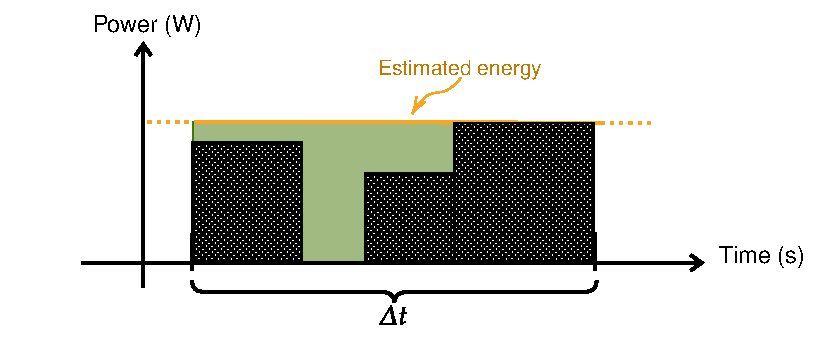
\includegraphics[scale=0.8]{Images/Model/energy_consumption.pdf}
    \caption{Energy consumption comparison between predicted and real. The black boxes are jobs. The green area is the energy predicted, but not used.}
    \label{fig:energy_consumption}
\end{figure}

The renewable production variation comes from the wind and solar variations. This variance comes from the uncertainties presented in Section \ref{sec:weather_uncertainties}. These uncertainties can increase or decrease power generation $P_{renew}$. Finally, the scheduling adaptations are scheduler changes to adapt the server configuration. Since the objective of the scheduling is to maximize the finished jobs, it must modify the offline plan. For example, if a job is running on a server, but the IT offline plan indicates putting this server to sleep, it would kill the job. So, ODM can change this decision, using more energy now and maintaining the job running. Another case is considering the speed given to the job. Letting a job in a server with a slower P-state can increase the execution time ($Ex_j$), violating Constraint \ref{equ:walltime} and killing the job. A way to reduce this possibility is by using Equation \ref{equ:avoid_walltime}. This equation verifies the minimum speed to complete the remaining job's flops. 

\begin{equation}
    (Wall_j - Ex_j) \times D_{s,d} \times F_{s,d} \ge Dfl'_j - Gfl_j
    \label{equ:avoid_walltime}
\end{equation}

Since ODM does not know the job's flops exactly, it can estimate using the walltime. Equation \ref{equ:estimated_job_size} shows a way for estimating $Dfl'_j$, similar to \cite{takizawa2020effect}. $F'_{s}$ is a fixed speed applied to the job. $\epsilon_{u}$ is a user error because the user can overestimate the execution time. \citeauthor{takizawa2020effect} calculate $\epsilon_{u}$ for each user, using previous users' requests. Even if Equation \ref{equ:avoid_walltime} does not exactly use the real size, it is a good way to balance the states of a job.

\begin{equation}
    \label{equ:estimated_job_size}
    Dfl'_j = wall_j \times F'_{s} \times \epsilon_{u}
\end{equation}

The batteries smooth these variations, providing the power needed in case of underproduction or absorbing the generation excess. At the end of time step $t$, the $SoC(t)$ can be different from the prediction. Therefore, ODM recalculates all future $SoC$ using Equations \ref{equ:battery_energy} and \ref{equ:battery_state_of_charge}. With the $SoC(T)$ updated, Equation \ref{equ:delta_energy} can estimate how far the SoC at the end of the time window will be from the target. A positive $\Delta E_{bat}$ means that the battery will have more energy than predicted, allowing the scheduler to use this excess to run more jobs or speed up the servers. On the other hand, a negative $\Delta E_{bat}$ means that the battery will have less energy than predicted. In this case, ODM must reduce future usage to approximate $SoC(T)$ to $SoC_{target}$.

\begin{equation}
    \label{equ:delta_energy}
    \Delta E_{bat} = \frac{SoC(T) - SoC_{target}}{100}\times B_{size}
\end{equation}

Then, ODM calculates how much energy it can compensate, using Equation \ref{equ:energy_battery}. This equation considers the loss in the process of charge/discharge. 

\begin{equation}
    \label{equ:energy_battery}
    E_{comp} = \begin{cases}
        \frac{\Delta E_{bat}}{\eta_{ch}} & \Delta E_{bat} > 0 \\
        \frac{\Delta E_{bat}}{\eta_{dch}} & \Delta E_{bat} < 0 \\
    \end{cases}
\end{equation}

Finally, ODM must modify futures $P_{dch}$ and $P_{ch}$ to use $E_{comp}$. We proposed some ways to deal with it in the following chapters. Since ODM modifies $P_{dch}$ and $P_{ch}$, $P_{prod}$ will also change (see Equation \ref{equ:model_energy}). So, ODM must adapt the IT plan (servers' states $D_{s,d}$) to meet the new $P_{prod}$. The algorithm to modify $D_{s,d}$ on-the-fly is also presented in the following chapters. This modification must respect the Constraint \ref{equ:ITDM_energy_less_envelope}.

\section{Data}
After describing the models, we describe the data used to simulate our environment. Our simulators expect three data: workload, weather, and platform. We explain the source of each one in the following sections. Section \ref{sec:simulation} details the adaptations to the simulation format.

\subsection{Workload Trace}
Workload trace is a log of job submissions in a resource (servers) provider. Some trace examples are Microsoft Azure \cite{cortez2017resource}, Google \cite{reiss2011google}, and Alibaba \cite{wang2022characterizing}. Regarding HPC, \citeauthor{feitelson2014experience} proposed the SWF format, which allows the data center providers to distribute logs to the research community \cite{feitelson2014experience}. In SWF, each line is a job with the fields separated by whitespace. Each line contains the following fields \cite{feitelson2014experience}:
\begin{itemize}
    \item \textit{Job Number}: The job ID starting with 1;
    \item \textit{Submit Time}: The submission time. The first job has 0 as submit time, and the following jobs use the first job as reference (in seconds);
    \item \textit{Wait Time}: How long the job waited in the queue (in seconds);
    \item \textit{Run Time}: The execution time in the data center (in seconds);
    \item \textit{Number of Allocated Processors}: The number of processors allocated to the job (integer);
    \item \textit{Average CPU Time Used}: The time that the job used the CPU. It is the average from all processors (integer);
    \item \textit{Used Memory}: The used memory, also average from all processors (kilobytes);
    \item \textit{Requested Number of Processors}: The number of processors requested by the user (integer);
    \item \textit{Requested Time}: This is the walltime (seconds);
    \item \textit{Requested Memory}: Requested memory per processor  (kilobytes);
    \item \textit{Status}: 1 if the job was completed, 0 if it failed, and 5 if canceled;
    \item \textit{User ID}: The user ID. Can be used to identify different jobs from the same user (integer);
    \item \textit{Group ID}: A group ID (some systems control the group and not the user ID) (integer);
    \item \textit{Executable (Application) Number}: Can link different jobs from the same application (integer);
    \item \textit{Queue Number}: Indicates in which queue the job was allocated (integer);
    \item \textit{Partition Number}: Indicates in which partition the job was allocated. For example, it is possible to use partition numbers to identify which machine in a cluster was used (integer);
    \item \textit{Preceding Job Number}: Indicates the number of a previous job in the workload, such that the current job can only start after the termination of this preceding job (integer);
    \item \textit{Think Time from Preceding Job}: The time between this job and the Preceding Job (seconds);
\end{itemize}

It is not mandatory to insert all information in a SWF file. Currently, Parallel Workloads Archive\footnote{https://www.cs.huji.ac.il/labs/parallel/workload/index.html} has 40 traces in SWF format. We chose the MetaCentrum2 workload trace from the Czech National Grid Organization \cite{klusavcek2015real}. MetaCentrum is a grid with resources in several cities in the Czech Republic. They have 19 clusters with 495 nodes and 8412 cores in total. The trace has 5,731,100 jobs from January 2013 to April 2015. Metacentrum does not provide the \textit{Average CPU Time Used}, \textit{Used memory}, \textit{Status}, \textit{Group ID}, \textit{Executable (Application) Number}, \textit{Preceding Job Number}, and \textit{Think Time from Preceding Job} fields. Metacentrum has different queues according to the job type. The Partition number indicates which cluster executed the job. We do not have much information about the servers, just the number of nodes, cores, and memory.

Figure \ref{fig:metacentrum} illustrates the inter-arrival and execution time distribution for MetaCentrum2. Inter-arrival is the time between job submissions, and execution time is the real runtime. Applying the Kolmogorov-Smirnov test to these data, we observed that both follow a log-normal distribution with p-value = 0.2174 for inter-arrival and p-value = 0.1802 for execution time (excluding 0.003838705\% of jobs as outliers).

\begin{figure}[!htb]
    \centering
    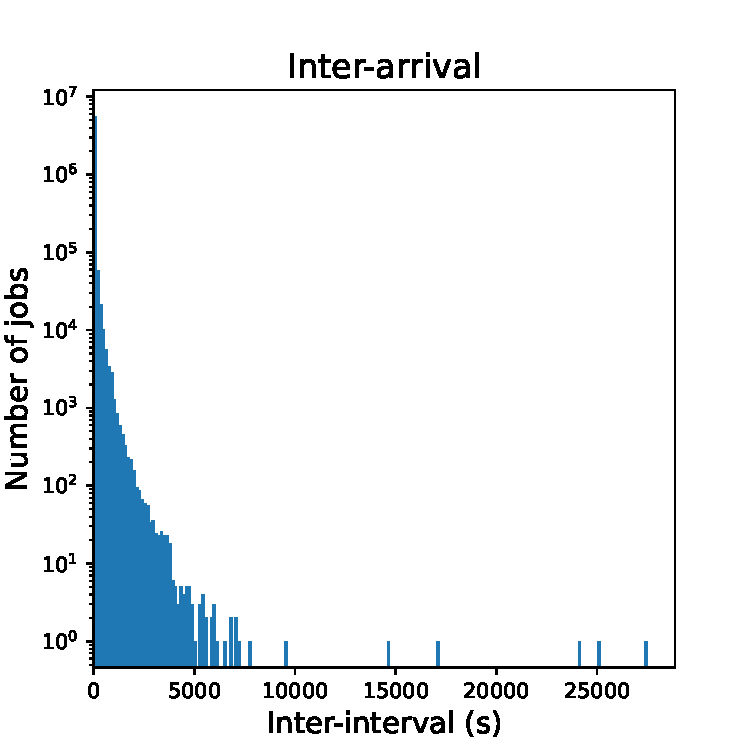
\includegraphics[scale=0.55]{Images/Model/interarrival.pdf}
    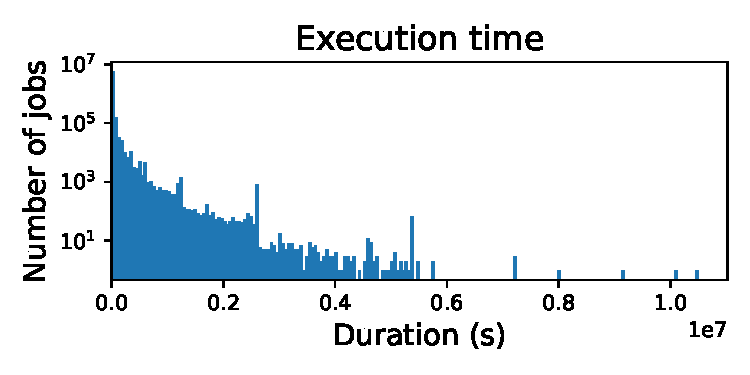
\includegraphics[scale=0.55]{Images/Model/execution_time.pdf}
    \caption{Inter arrival and execution time distribution for MetaCentrum2 workload trace.}
    \label{fig:metacentrum}
\end{figure}

We created two scripts for translating the SWF format to the BATSIM simulator and Datazero2 Middleware formats (we will present them in Section \ref{sec:simulation}). We simulated several possibilities of workload, and each chapter will describe the selection process.

\subsection{Weather Trace}

Regarding weather, we are interested in the traces of solar irradiance and wind speed, which allow us to estimate power generation using Equations \ref{equ:panel_solar_with_temperature} and \ref{equ:wind_turbines}. NASA's Modern-Era Retrospective Analysis for Research and Applications (MERRA) provides a dataset of solar irradiance and wind speed from any place in the world \cite{rienecker2011merra}. Regarding wind, we get the data directly from the MERRA site\footnote{https://power.larc.nasa.gov/data-access-viewer/}. Renewable Ninja\footnote{https://www.renewables.ninja/} is a tool that transforms the weather from MERRA to electricity production \cite{pfenninger2016long, staffell2016using}. Renewable Ninja uses some solar panel models to estimate power generation. We use Renewable Ninja to obtain ground-level solar irradiance because the authors consider cloud cover and aerosols. We chose Toulouse, France as the reference point, getting the data from 2020. After exporting the data, we also translate the output CSV to the BATSIM simulator and Datazero2 Middleware formats. As for the workload, we took different days from 2020 for our simulations. The following chapters will present the selection process.

\subsection{Platform Configuration}

Finally, the last data is the hardware specification. This configuration simulates the real behavior of the different components of a data center, such as servers, storage, network, etc. In this thesis, we focused on the server specification. For simulating a DVFS-enabled server, the following information is necessary:
\begin{itemize}
    \item Sleeping power: Power used to maintain a server sleeping;
    \item Time for on\(\rightarrow\)off transition: Time to turn off a server;
    \item Power for on\(\rightarrow\)off transition: Power to turn off a server;
    \item Time for off\(\rightarrow\)on transition: Time to turn on a server;
    \item Power for off\(\rightarrow\)on transition: Power to turn on a server;
    \item Power idle: Power used when the server is idle;
    \item DVFS states: A list of states containing:
    \begin{itemize}
        \item Power: The power used in the state with all processors busy;
        \item Speed: The speed in the state.
    \end{itemize}
\end{itemize}

We chose to model a data center using the specification from GRID5000 servers. \citeauthor{dacosta:hal-03453537v1} performed experiments in GRID5000 to obtain the data for the DVFS states \cite{dacosta:hal-03453537v1, dacostakeynote}. Some other authors also simulated GRID5000 machines, giving information about their simulation \cite{rais2018quantifying, caux2018optimization, caux2019phase, villebonnet2016energy}. We consolidate these works to create a platform for both the BATSIM simulator and Datazero2 Middleware. Table \ref{tab:gros} exemplifies the consolidated data for GRID5000's Gros server used in the experiments.

% \begin{table}[!htb]
% \centering
% \caption{Gros definition. The power is for all server's processors busy. The values are from Grid5000's Gros server.}
% \label{tab:gros}
% \begin{tabular}{ll|l}
%     \hline
%     \multicolumn{2}{l|}{Parameter} & Value \\ \hline\hline
%     \multicolumn{2}{l|}{Sleeping power} & 4.5 W \\
%     \multicolumn{2}{l|}{Time on-\textgreater{}off} & 6 s \\
%     \multicolumn{2}{l|}{Power on-\textgreater{}off} & 76.5 W \\
%     \multicolumn{2}{l|}{Time off-\textgreater{}on} & 164 s \\
%     \multicolumn{2}{l|}{Power off-\textgreater{}on} & 110.52 W \\
%     \multicolumn{2}{l|}{Power idle} & 62 W \\ \hline
%     \multicolumn{3}{l}{DVFS states}  \\ \hline 
%     \multicolumn{1}{l|}{State} & Power (W) & Speed per core (Gflops) \\ \hline\hline
%     \multicolumn{1}{l|}{0} & 143.45 & 35.2 \\
%     \multicolumn{1}{l|}{1} & 123.57 & 33.59 \\
%     \multicolumn{1}{l|}{2} & 122.34 & 31.98 \\
%     \multicolumn{1}{l|}{3} & 121.68 & 30.36 \\
%     \multicolumn{1}{l|}{4} & 118.49 & 28.79 \\
%     \multicolumn{1}{l|}{5} & 115.8 & 27.14 \\
%     \multicolumn{1}{l|}{6} & 114.58 & 25.57 \\
%     \multicolumn{1}{l|}{7} & 110.89 & 23.85 \\
%     \multicolumn{1}{l|}{8} & 108.06 & 22.38 \\
%     \multicolumn{1}{l|}{9} & 106.81 & 20.78 \\
%     \multicolumn{1}{l|}{10} & 104.13 & 19.18 \\
%     \multicolumn{1}{l|}{11} & 102.83 & 17.59 \\
%     \multicolumn{1}{l|}{12} & 100.78 & 15.99 \\ \hline
% \end{tabular}
% \end{table}

\begin{table}[!htb]
    \caption[Gros definition]{Gros definition. The power is for all server's processors busy. The values are from Grid5000's Gros server.}
    \label{tab:gros}
    \begin{minipage}{.45\linewidth}
      \centering
      \begin{tabular}{l|l}
        \hline
        Parameter & Value \\ \hline\hline
        Sleeping power & 4.5 W \\
        Time on$\rightarrow$off & 6 s \\
        Power on$\rightarrow$off & 76.5 W \\
        Time off$\rightarrow$on & 164 s \\
        Power off$\rightarrow$on & 110.52 W \\
        Power idle & 62 W \\ \hline
    \end{tabular}
    \end{minipage}%
    \begin{minipage}{.55\linewidth}
      \centering
      \begin{tabular}{l|l|l}
        \hline
        State & Power (W) & Speed per core (Gflops) \\ \hline\hline
        0 & 143.45 & 35.2 \\
        1 & 123.57 & 33.59 \\
        2 & 122.34 & 31.98 \\
        3 & 121.68 & 30.36 \\
        4 & 118.49 & 28.79 \\
        5 & 115.8 & 27.14 \\
        6 & 114.58 & 25.57 \\
        7 & 110.89 & 23.85 \\
        8 & 108.06 & 22.38 \\
        9 & 106.81 & 20.78 \\
        10 & 104.13 & 19.18 \\
        11 & 102.83 & 17.59 \\
        12 & 100.78 & 15.99 \\ \hline
    \end{tabular}
    \end{minipage} 
\end{table}

\section{Simulation}
\label{sec:simulation}

After describing the source of data, we detail our simulation environment. We explain two simulators and the work done to adapt our data for these simulators. Also, we define the different metrics used to evaluate the algorithms in the following chapters.

\subsection{BATSIM Simulator}


\subsection{Datazero2 Middleware}
% Explain about docker

\subsection{Metrics}

\section{Conclusion}